\documentclass{article}

\usepackage{fontspec}   %加這個就可以設定字體

\usepackage{lingmacros}
\usepackage{amssymb,amsmath,amsthm, mathtools}
\usepackage{graphicx}
\newtheorem{theorem}{Theorem}
\newtheorem*{theorem*}{Theorem}
\newtheorem*{remark}{Remark}
\usepackage{indentfirst}
\usepackage{tikz}

\begin{document}
\title{Iterative Method For Linear System - Report}
\author{NTU CSIE \& MATH Jerry Chou}
\date{2014/11/24}
\maketitle

\section{Homework Description}
\paragraph{}
In this homework, we are going to use four iterative methods to solve two kind of sparse linear system with different scales. The four iterative methods are:
\begin{itemize}
\item Gauss-Seidel
\item PCG with identity matrix as preconditioner
\item PCG with incomplete Cholesky matrix as preconditioner (iPCG)
\item Symmetric Gauss-Seidel (sym-Gauss-Seidel)
\end{itemize}

\paragraph{}
There are two type of input linear system in this homework. The first problem is that the matrix is regular and the other is refined at a hole. For each method, we tried three cases with type 1 and 2 cases with type 2. On the other hand, we focus on the following features in the result:
\begin{itemize}
\item Elapsed time
\item Storage
\item Number of iterations
\end{itemize}


% Result
\newpage
\section{Result}

We compare three important features between the four methods we use. The features are: number of iterations, elapsed time, and storage. The result of the first category dataset is as follow:
\begin{figure}[ht!]
\centering
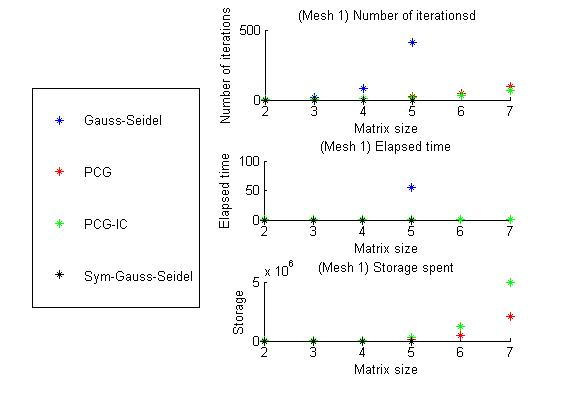
\includegraphics[width=120mm]{mesh1result.jpg}
\caption{Result using mesh 1 dataset}
\label{overflow}
\end{figure}


% Analysis on nuber of iterations
\subsection{Number of iterations} 
\paragraph{}
First, let's take a look at the number of iterations using four different iterative linear system solving method:
\begin{table}[h]
\begin{center}
\begin{tabular}{lcccc}
\hline
Method & Size = 9 & Size = 49 & Size = 225 & Size = 961\\
\hline
Gauss-Seidel & 3 & 17 & 85 & 411\\
PCG & 2 & 10 & 10 & 23\\
iPCG & 2 & 3 & 9 & 17\\
sym-Gauss-Seidel & 3 & 14 & 67 & 321\\
\hline
\end{tabular}
\caption{Number of iterations using four iterative methods}
\end{center}
\end{table}

\paragraph{}
We can easily see that no matter using Gauss-Seidel or symmetric Gauss-Seidel method to solve iterative linear system, the number of iterations will quickly increases.
If we look more deep inside the algorithm of Gauss-Seidel method, we know that the iteration rule of it is as follow:
$$x^{(k+1)} = (D+L)^{-1}Ux^{(k)} + (D+L)^{-1}b$$

\paragraph{}
Recall that the convergence rate of stationary iterative method will be same as the convergence rate of $\|B\|$ to zero, where $B$ is the iteration matrix. Also, the convergence rate of $\|B\|$ to zero is equal to the convergence rate to zero of $B$ 's top eigenvalue $\lambda_{max}$. Using $Matlab$ to calculate the absolute value of the top eigenvalue of the iteration matrices of each size. 
\begin{table}[h]
\begin{center}
\begin{tabular}[c]{lccc}
\hline
 & Size = 9 & Size = 49 & Size = 225 \\
\hline
$\lambda_{max}$ & -0.509587 & -0.854224& -0.961987 \\
\hline
\end{tabular}
\caption{top eigenvalue of the iteration matrices}
\end{center}
\end{table}

\paragraph{}
On the other hand, we know the bond on the error after $k$ iterations of the PCG algorithm:\cite[pp.155-156]{QSS07}
$$\|x^{(k)}-x^*\|_A \leq \frac{2c^k}{1+c^{2k}}\|x^{(0)}-x^*\|_A$$
where
$c = \frac{\sqrt{\kappa(A)}-1}{\sqrt{\kappa(A)}+1}$
\paragraph{}
This is a tighter upper bound for iteration error than the upper bound given in the homework description.
$$\|x^{(k)}-x^*\|_A \leq 2(\frac{\sqrt{\kappa(A)}-1}{\sqrt{\kappa(A)}+1})^k\|x^{(0)}-x^*\|_A$$

\paragraph{}
I found some paper claiming that the rate of convergence of PCG with some specific algorithm in certain cases are quadratic. However, the proof is a little bit difficult for me. A result I found in one paper\cite{CG} seems more reasonable, although it is also a loose upper bound. 

\begin{figure}[h]
\centering
\includegraphics[width=40mm]{convergence_CG_1.png}
\caption{Convergence of Conjugate Gradients (per iteration) as a function of condition number}
\label{overflow}
\end{figure}

\paragraph{}
Also, let's calculate the condition number of iteration matrices of different size. The result is as follow:
\begin{table}[h]
\begin{center}
\begin{tabular}{lcccc}
\hline
Method & Size = 9 & Size = 49 & Size = 225 & Size 961 \\
\hline
& 9.000 & 37.265 & 150.417 & 603.052\\
\hline
\end{tabular}
\caption{Condition Number of iteration matrices with different size}
\end{center}
\end{table}

\paragraph{}
Consider the iteration matrix with size = 225. Using extrapolation to estimate the convergence rate per iteration is about $0.83$. From Table 2, the convergence rate of same system with Gauss-Seidel method is $0.96$. Thus we can calculate the ratio of the number of iterations between the two methods at the same error level. The result is $\frac{\log0.96}{\log0.83} = 0.2191$, which is closed to the ratio of real number of iterations: $\frac{10}{85} = 0.1176$

\paragraph{}
After comparing the the convergence rate of Gauss-Seidel and PCG, we can learn that the convergence rate of PCG is far more faster than Gauss-Seidel when the iteration will converge.

\paragraph{}
In the end of the discussion about number if iterations, let's consider only using PCG method with preconditioner to be identity matrix and incomplete Cholesky matrix. Since these two methods are relatively fast, I will increase the size of the linear system and how the number of iterations change.
\begin{table}[h]
\begin{center}
\begin{tabular}{lcccccc}
\hline
Method & 9 & 49 & 225 & 961 & 3969 & 16129\\
\hline
PCG & 2 & 10 & 10 & 23 & 47 & 95\\
iPCG & 2 & 3 & 9 & 17 & 32 & 66\\
\hline
\end{tabular}
\caption{Number of iterations using PCG and iPCG iterative methods. The first row is the size of the linear system.}
\end{center}
\end{table}



% Analysis on Elapsed time
\subsection{Elapsed Time}
In the beginning, let's take a look at the elapsed time using four different iterative linear system solving method:
\begin{table}[h]
\begin{center}
\begin{tabular}{lcccc}
\hline
Method & Size = 9 & Size = 49 & Size = 225 & Size = 961\\
\hline
Gauss-Seidel & 0.0007 & 0.0224 & 0.5724 & 18.1756\\
PCG & 0.0002 & 0.0002 & 0.0010 & 0.1012\\
iPCG & 0.0001 & 0.0354 & 0.0005 & 0.1253\\
sym-Gauss-Seidel & 0.0021 & 0.0354 & 0.9260 & 28.1574\\
\hline
\end{tabular}
\caption{Elapsed time using four iterative methods}
\end{center}
\end{table}
\paragraph{}
The elapsed time is proportional to the number of iterations and system size since the iterating time per iterations is linear to the size of the iteration matrix or vector.


% Analysis on Storage
\subsection{Storage}
The storages used in different size of linear system with each iterative method are listed as follow:


% Reference
\renewcommand\refname{Reference}
\bibliographystyle{plain}
\bibliography{Thesis}

\end{document}
